\documentclass[12pt, a4paper]{article}
\usepackage{tikz}
\usepackage{float}
\usepackage{graphicx}
\usepackage{pgfplots}
\usepackage{amsmath}
\makeatletter
\def\@fnsymbol#1{\ensuremath{\ifcase#1\or 1\or 2\or
		3\or \mathparagraph\or \|\or **\or \dagger\dagger
		\or \ddagger\ddagger \else\@ctrerr\fi}}
\makeatother
\usepackage[italian]{babel}
\title{Variazione di pressione in relazione all'Eruzione del vulcano presso  \emph{Hunga Tonga}\\ \Large{Stazione Meteorologica Open Source}}
\author{Mattia Mascarello\thanks{m2.mascarello@liceococito.it}\and Lorenzo Dellapiana\thanks{l.dellapiana@liceococito.it}\and Luca Savio Biello\thanks{ls.biello@liceococito.it}}
\date{\parbox{\linewidth}{\centering%
		\today\endgraf\bigskip
		Liceo Scientifico Statale ``Leonardo Cocito''}}
\begin{document}
	
	\maketitle
	
	\begin{abstract}
		Il giorno 15 gennaio 2022, alle ore 5 (Ora locale di Roma, o 17, ora locale di Tonga) il vulcano \emph{Ha’apai}, ubicato a circa $65Km$ dalla capitale di Tonga, \emph{Nuku’alofa}, è stato il teatro di una violenta euruzione, che ha gnerato una colonna di polveri alta $30 Km$ ed un'onda d'urto rilevabile in tutto il mondo come una variazione di pressione attraverso le stazioni meteorologiche lì dislocate.\\
		In questo articolo analizziamo i dati ricevuti dalla nostra stazione e stabiliamo la compatibilità temporale dell'evento vulcanologico con le misurazioni da noi effettuate, che risultano coincidenti alle previsioni.
	\end{abstract}
	\pagebreak
	\tableofcontents
	\pagebreak
\section{Propagazione dell'urto e modello probabilistico}
	
\begin{figure}[H]
	\centering
	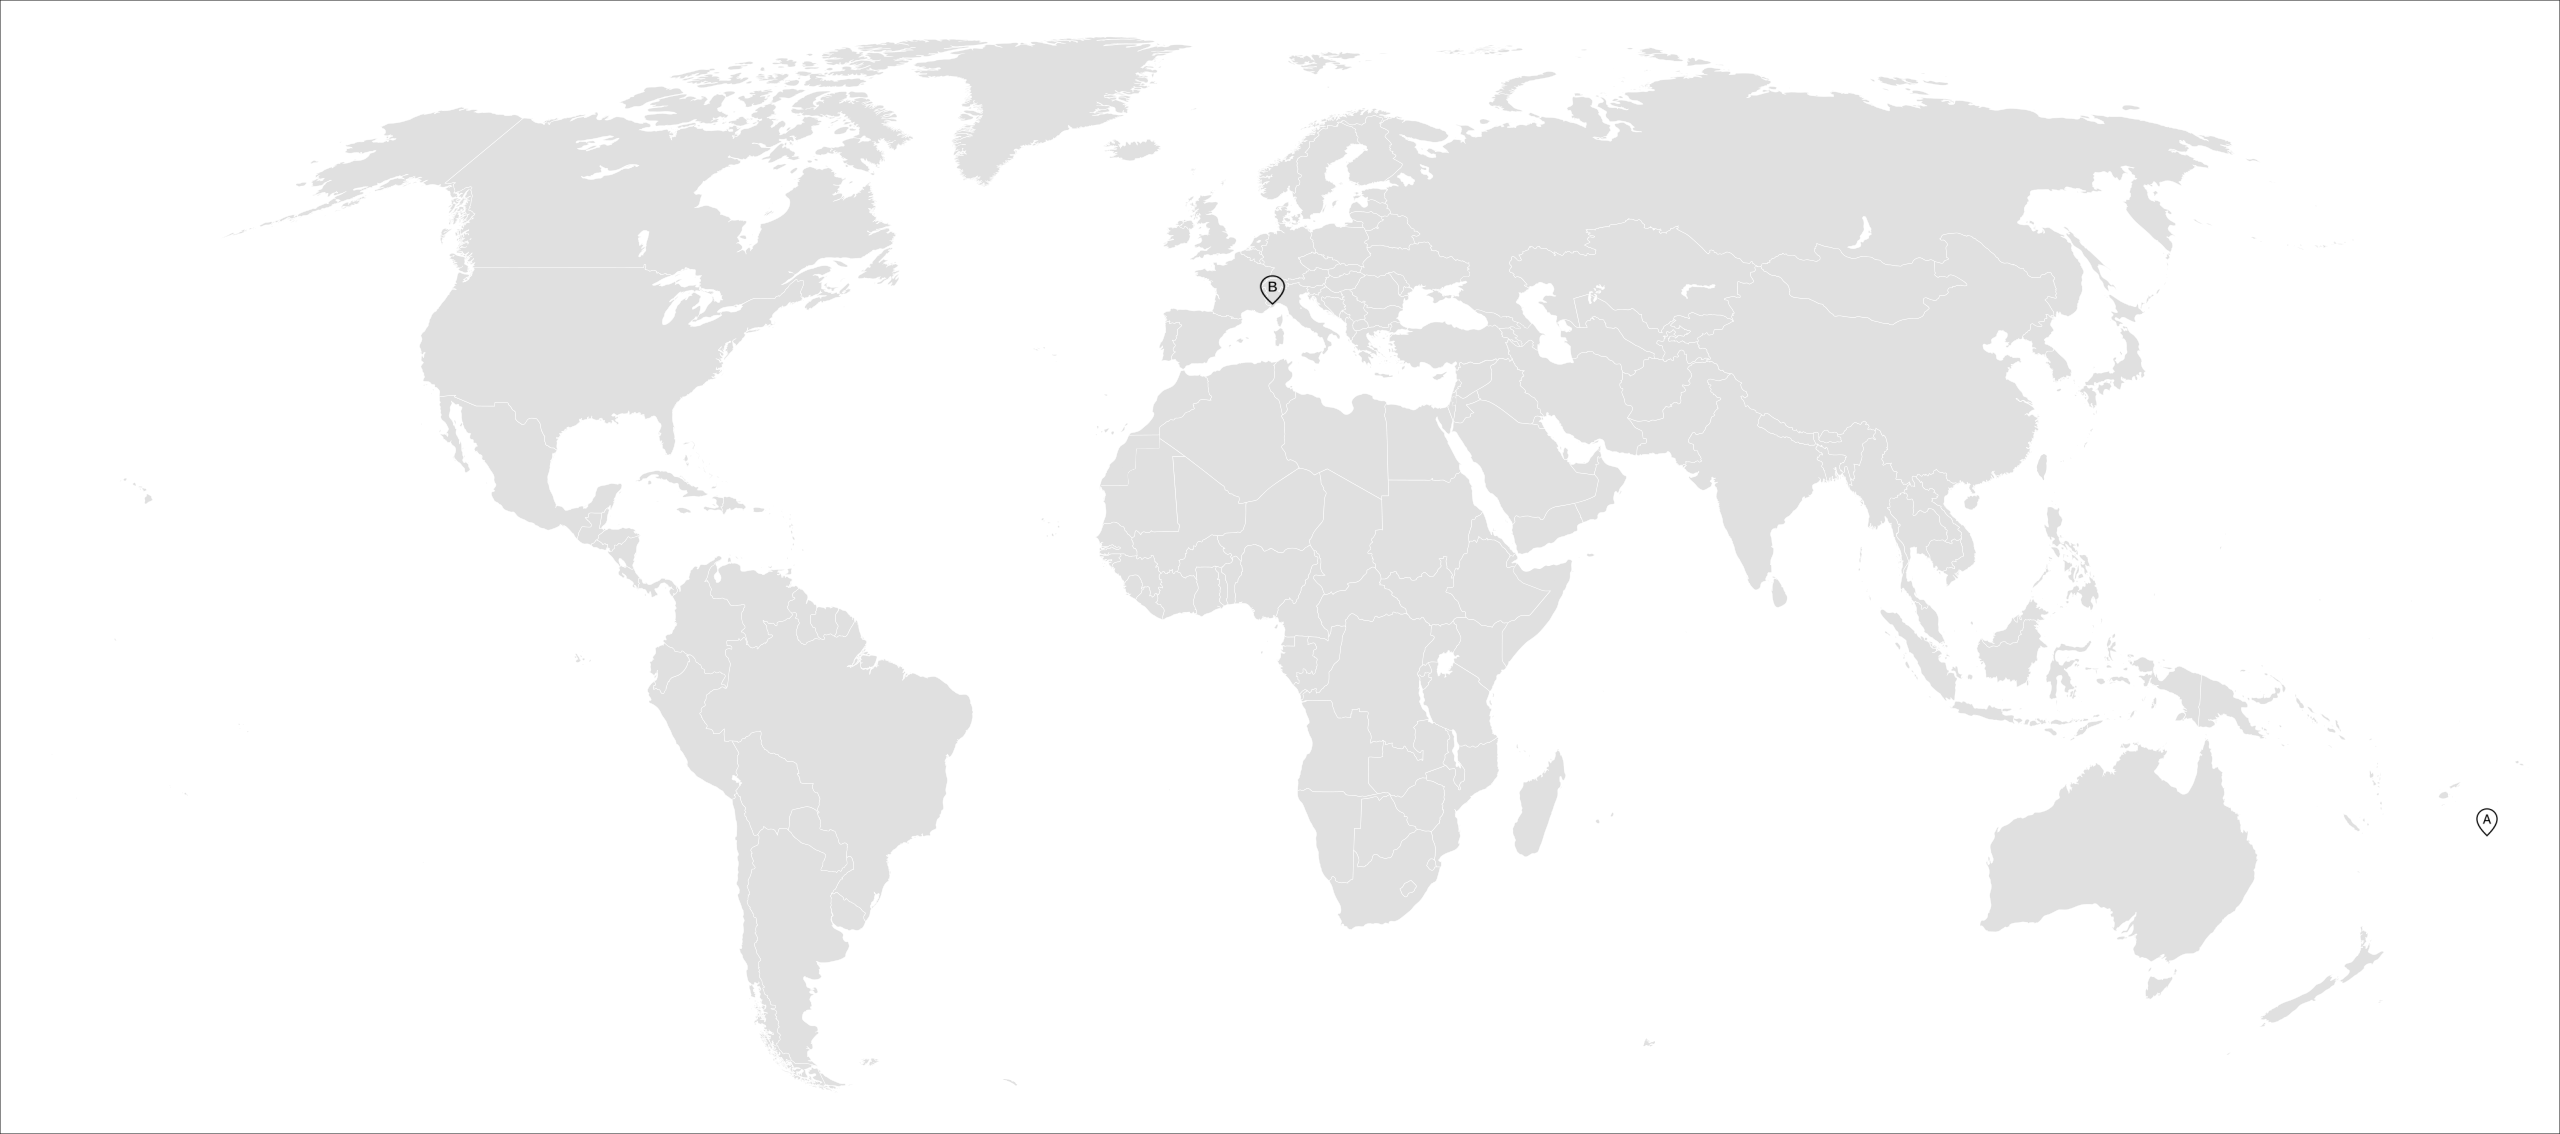
\includegraphics[width=\textwidth]{wmab.png}
	\caption{Planisfero con marcatori posizionali}
\end{figure}
\begin{figure}[H]
	\centering
	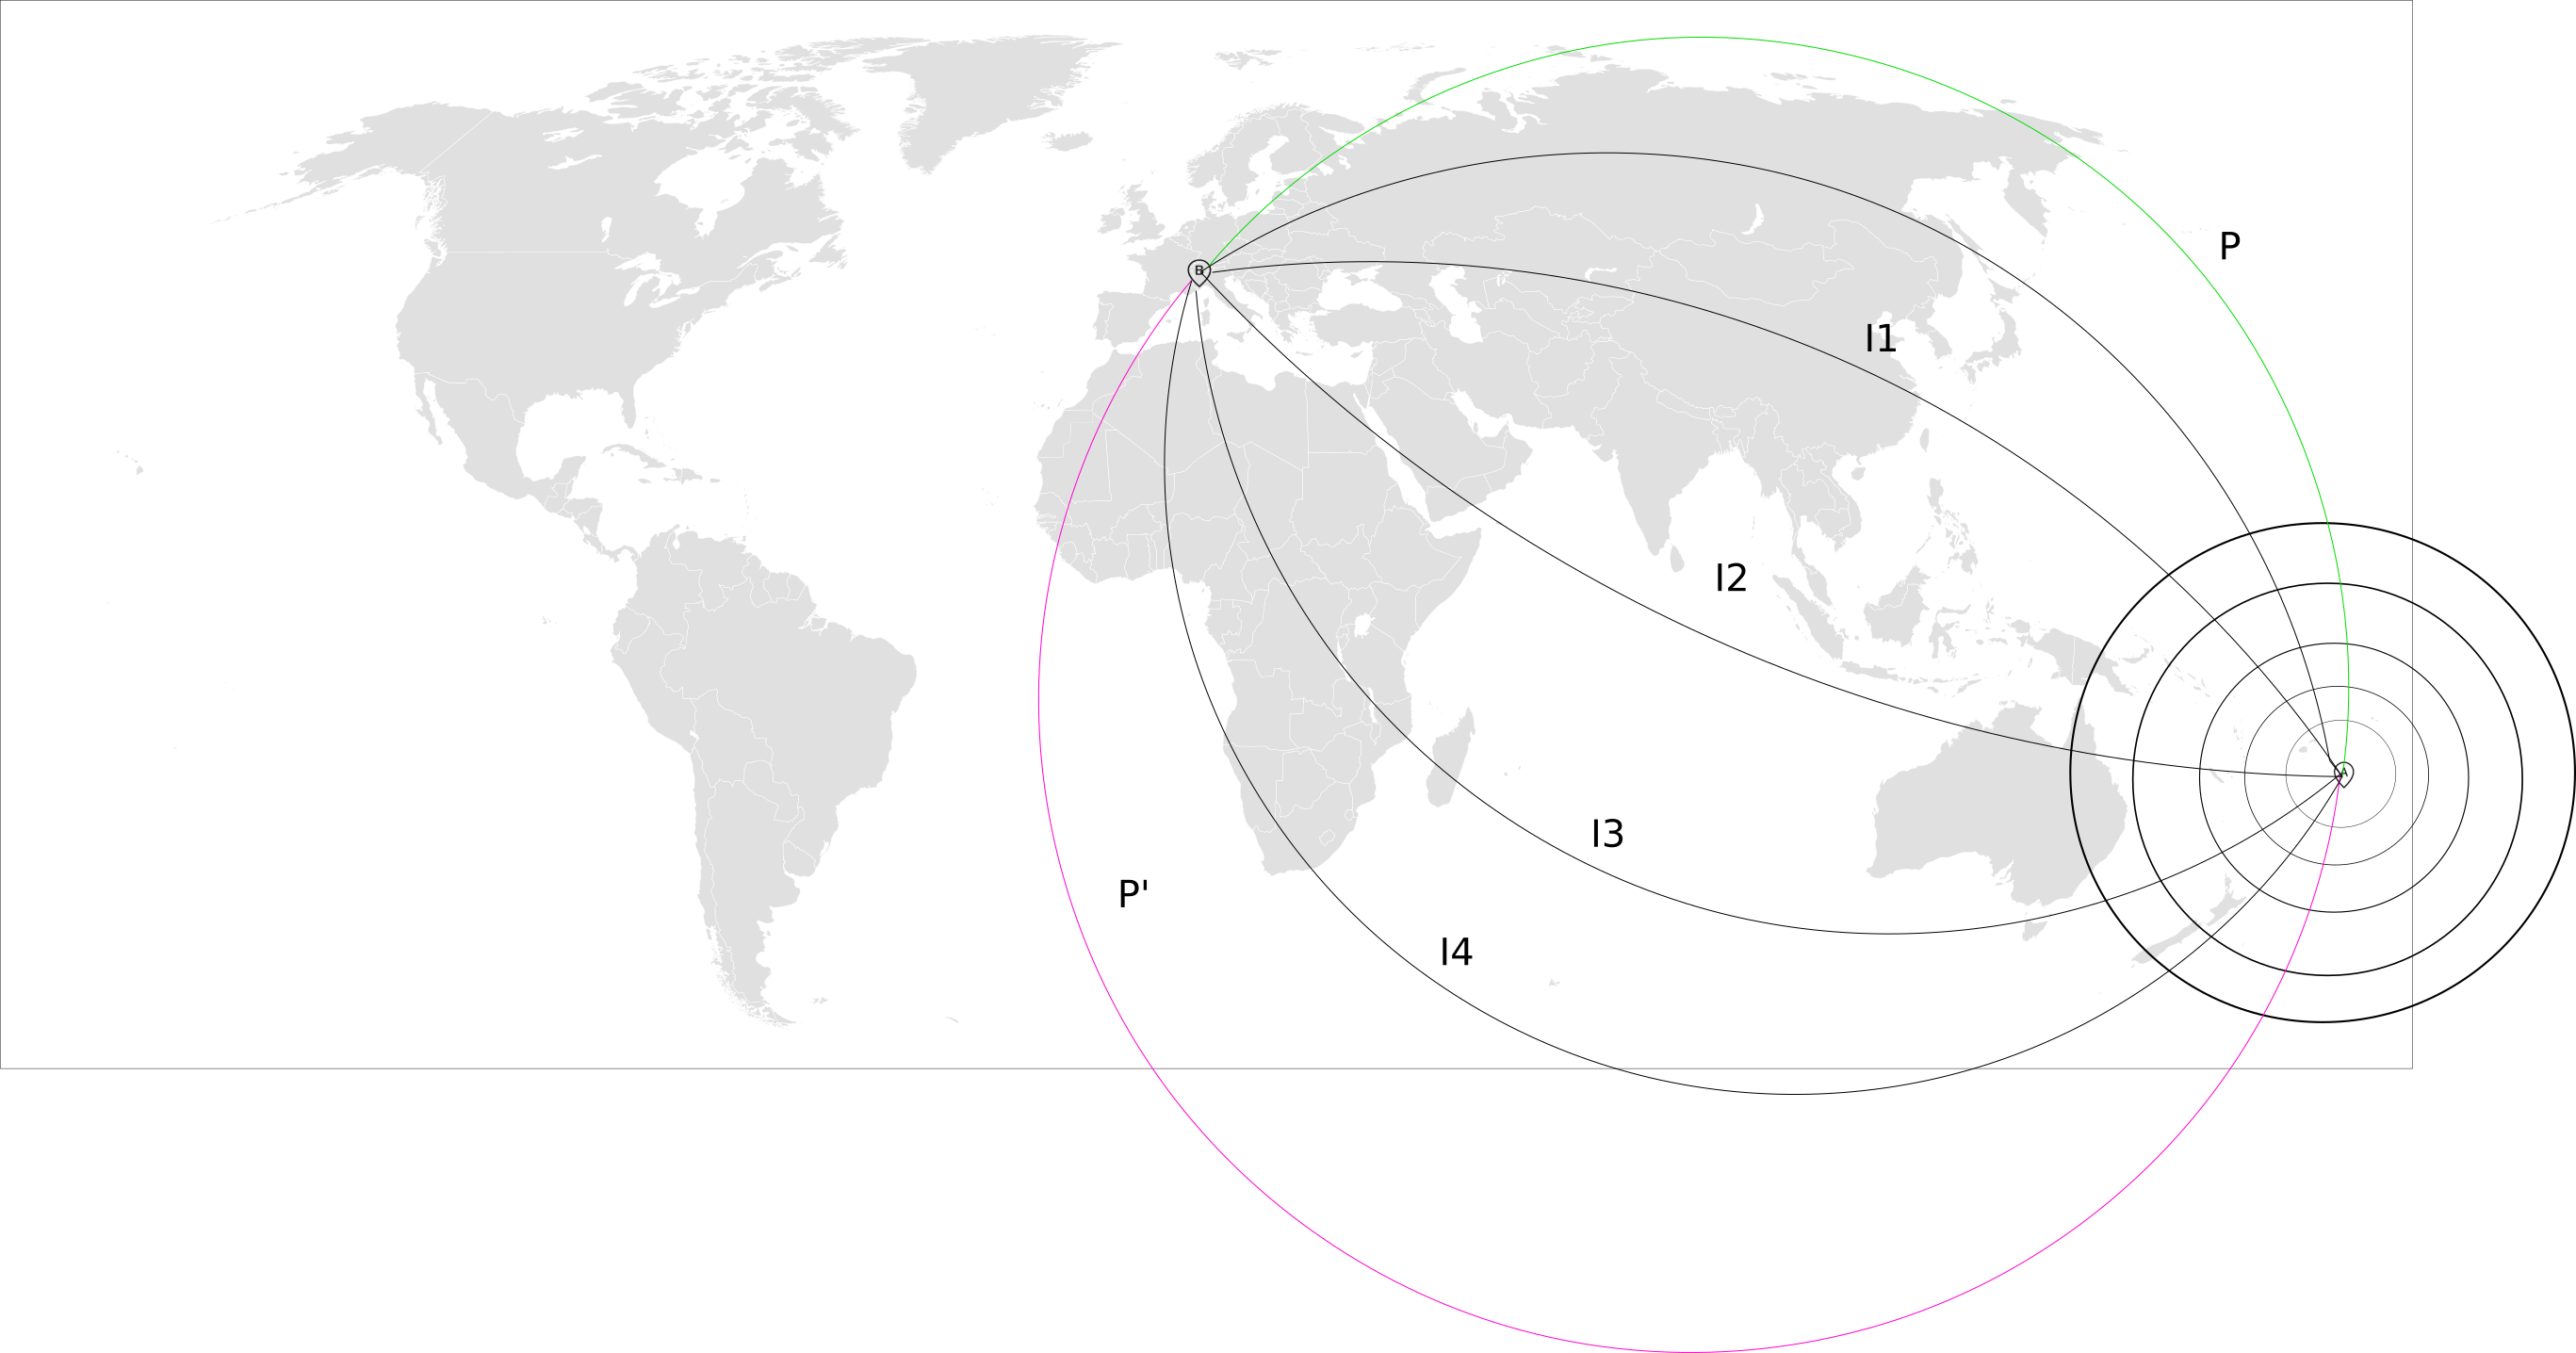
\includegraphics[width=1.08\textwidth]{wmi.png}
	\caption{Percorso dell'onda d'urto}
\end{figure}
Sussistono infiniti perscorsi percorribili dall'onda d'urto causata dall'eruzione (che è qui modellizzata come sorgente puntiforme $A$ che trasmette l'urto in tutte le direzioni in modo equipollente), di cui $P$ è quello più breve, $P'$ quello più esteso ($I_n$ rappresentano alcune enumerazioni di percorsi intermedi).

L'aumento della pressione atmosferica rilevabile in un punto sulla superficie terrestre (in questo caso $B$ contrassegna la nostra stazione) è misurabile come la sommatoria delle forze esercitate dalle onde d'urto provenienti da tutte le direzioni percorrribili che in quel momento stanno transitando presso il punto interessato.

Le onde provenienti dal percorso $P$ sono le prime a sopraggiungere, seguite da tutte le altre fino a $P'$ che impiega il tempo massimo per raggiungere il sito di misurazione.

Si può quindi assumere che nell'intervallo tra questi due estremi il transito delle onde segua una distribuzione gaussiana come segue



\pgfmathdeclarefunction{gauss}{2}{%
	\pgfmathparse{1/(#2*sqrt(2*pi))*exp(-((x-#1)^2)/(2*#2^2))}%
}
\begin{figure}[H]
	\centering
\begin{tikzpicture}
	\begin{axis}[
		no markers, 
		domain=0:6, 
		samples=100,
		axis lines*=left, 
		xlabel=$x$,
		every axis y label/.style={at=(current axis.above origin),anchor=south},
		every axis x label/.style={at=(current axis.right of origin),anchor=west},
		height=5cm, 
		width=12cm,
		xtick=\empty, 
		ytick=\empty,
		enlargelimits=false, 
		clip=false, 
		axis on top,
		grid = major
		]
		
		\addplot [very thick,black!50!black] {gauss(3, 1)};
	
		
		
	\end{axis}
	
	\node[below] at (1, 0)  {$P$}; 
	\node[below] at (3, 0)  {$I_1$};
	\node[below] at (5, 0)  {$I_2$};
	\node[below] at (7, 0)  {$I_3$};
	\node[below] at (9, 0)  {$I_4$};
	\node[below] at (10, 0)  {$P'$}; 
	
	
\end{tikzpicture}
	\caption{Distribuzione delle onde d'urto in transito}
\end{figure}

Appurato questo è possibile calcolare l'istante di arrivo di $P$ e $P'$, avvalendosi della velocità del suono (costante nota) e quindi determinare la media aritmetica tra i due istanti ottenuti per determinare la previsione di massimo $\Delta P$.

\section{Calcolo degli istanti di arrivo}
Si assumono i seguenti valori
\begin{center}
\begin{tabular}{|c|c|c|}
	\hline
	Luogo & Latitidine & Longitudine \\
	\hline
	\hline
	Alba (CN) & 44°41'33"00 N & 08°1'36"12 E \\
	\hline
	Tonga & 21° 10' 44.3496'' S & 175° 11' 53.6712'' W \\
	\hline
\end{tabular}
\end{center}
L'altitudine è ritenuta trascurabile
\subsection{$P$ (minimo)}
La minima distanza tra $A$ e $B$ è calcolabile con la formula dell'eminoverso.\\
Assumendo per la città di \textbf{Alba} \begin{equation*}\begin{cases}lat=\varphi_1\\lon=\lambda_1\end{cases}\end{equation*}
e per \textbf{Tonga} \begin{equation*}\begin{cases}lat=\varphi_2\\lon=\lambda_2\end{cases}\end{equation*}

E dopo aver definito

$$
{\displaystyle \operatorname {hav} (\theta )=\sin ^{2}\left({\frac {\theta }{2}}\right)={\frac {1-\cos(\theta )}{2}}}
$$

La distanza $d$ è calcolabile come

$$
{\displaystyle {\begin{aligned}d&=2r\arcsin \left({\sqrt {\operatorname {hav} (\varphi _{2}-\varphi _{1})+(1-\operatorname {hav} (\varphi _{1}-\varphi _{2})-\operatorname {hav} (\varphi _{1}+\varphi _{2}))\cdot \operatorname {hav} (\lambda _{2}-\lambda _{1})}}\right)\\&=2r\arcsin \left({\sqrt {\sin ^{2}\left({\frac {\varphi _{2}-\varphi _{1}}{2}}\right)+\left(1-\sin ^{2}\left({\frac {\varphi _{2}-\varphi _{1}}{2}}\right)-\sin ^{2}\left({\frac {\varphi _{2}+\varphi _{1}}{2}}\right)\right)\cdot \sin ^{2}\left({\frac {\lambda _{2}-\lambda _{1}}{2}}\right)}}\right)\\&=2r\arcsin \left({\sqrt {\sin ^{2}\left({\frac {\varphi _{2}-\varphi _{1}}{2}}\right)+\cos \varphi _{1}\cdot \cos \varphi _{2}\cdot \sin ^{2}\left({\frac {\lambda _{2}-\lambda _{1}}{2}}\right)}}\right)\approx \boxed{17314 Km}\end{aligned}}}
$$

È noto che a 20°C $v_{suono_{aria}}=343\frac{m}{s}=1238\frac{Km}{h}$.

Quindi, conosciuta la lunghezza $d$ di $P$ e la velocità di propagazione del suono si calcola il tempo impiegato per sopraggiungere ad Alba.
$$
t_P=\frac{d}{v}=\frac{17314Km}{1238\frac{Km}{h}}=13,98h\approx14h
$$

\subsection{$P'$ (massimo)}

Giacchè la Terra è assimilabile ad una sfera siccome il raggio e quindi la circonferenza si discostano in modo trascurabile (ai fini del presente articolo) dalla media dei valori in tutti i punti del globo, è possibile calcolare il massimo percorso come 
$$
d'=C-d=40041Km-17314Km=22727Km
$$

Possiamo quindi nuovamente calcolare

$$
t_{P'}=\frac{d'}{v}=\frac{22727Km}{1238\frac{Km}{h}}=18,35h\approx18h
$$
\subsection{$R$ (medio)}

Il tempo di percorrenza medio (\emph{cfr 1.}) è quindi

$$
t_m=\frac{h+h'}2=\frac{18h+14h}2=16h
$$

E l'ora finale di arrivo è quindi

$$
h_f=h_i+t_m=5+16=21h
$$


In cui la nostra stazione meteo ha rilevato una repentina variazione di pressione nell'intervallo
$$
I_P=[1006,1009]hPa
$$

Dalle ore 20:58 alle ore 21:01.
\end{document}